
En este problema, usted encontrará una situación en la cual un espejo plano proporciona una imagen real. El espejo cóncavo E, que se muestra en la figura de este problema, proporcionaría la imagen I del objeto O si el espejo plano E' no interrumpiese la trayectoria de los rayos luminosos reflejados por E. En esas condiciones estos rayos luminosos inciden sobre E' y vuelven a reflejarse.
\begin{enumerate}
    \item La figura muestra dos rayos luminosos que inciden sobre E'. Trace en el diagrama la trayectoria de estos rayos luego de ser reflejados por E'.
    \item Obtenga luego, la imagen I' del objeto O proporcionada ahora por E'.
    \item ¿Esta imagen es real o virtual?
\end{enumerate}

\begin{figure}[h!]
    \centering
    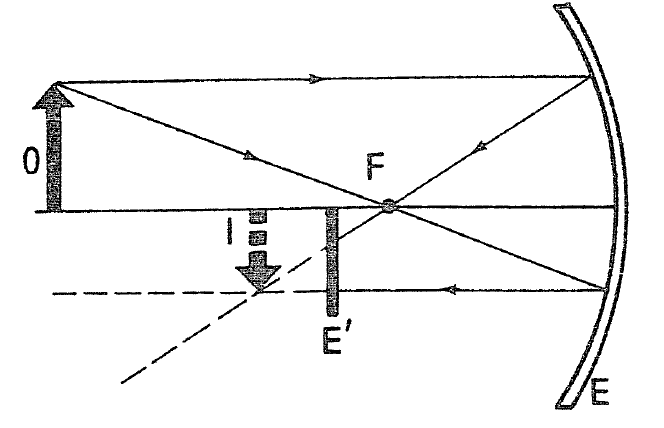
\includegraphics[scale=0.4]{enunciados/alvarenga_p649_16.png}
    \caption{Alvarenga p. 649 - Ejercicio 16}
\end{figure}
